\documentclass[]{article}

% Imported Packages
%------------------------------------------------------------------------------
\usepackage{amssymb}
\usepackage{amstext}
\usepackage{amsthm}
\usepackage{amsmath}
\usepackage{enumerate}
\usepackage{fancyhdr}
\usepackage[margin=1in]{geometry}
\usepackage{graphicx}
\usepackage{float}
\usepackage{extarrows}
\usepackage{setspace}
%------------------------------------------------------------------------------

% Header and Footer
%------------------------------------------------------------------------------
\pagestyle{fancy}  
\lhead{T2 Group 10}
\chead{Detailed Design}
\rhead{SFWRENG 3A04}
\renewcommand\headrulewidth{0.4pt}                  
\renewcommand\footrulewidth{0.4pt}                                        
%------------------------------------------------------------------------------

% Title Details
%------------------------------------------------------------------------------
\title{\textbf{Boardzilla\break Detailed Design}}
\author{Matthew Paulin \\ paulinm \\ 400187147 \and
        Hargun Bedi \\ bedih \\ 400185463 \and
        Dylan Smith \\ smithd35 \\ 001314410 \and
        Chenwei Song \\ songc12 \\ 400124879 \and
        Tianzheng Mai \\ mait6 \\ 400143042
}
\date{\today}                                
%------------------------------------------------------------------------------

% Document
%------------------------------------------------------------------------------
\begin{document}

\maketitle	

\section{Introduction}
\label{sec:introduction}
% Begin Section
\subsection{Purpose}
\label{sub:purpose}
% Begin SubSection
The purpose of this document is to identify the major components of the system and describe their interactions. The information is presented in the form of detailed diagrams of Boardzilla including state charts for controller classes, sequence diagrams, and a detailed class diagram. Through these diagrams, the reader should have a good understanding of how the system functions and how transitions are handled. The target audience includes the professor and teaching assistants who will inspect the document as well as the developers who may use this document as a reference.
% End SubSection

\subsection{System Description}
\label{sub:system_description}
% Begin SubSection
Boardzilla is an online application that serves as a dashboard for a variety of information meant to serve as a daily briefing or hub. Each user will have their own protected account with a customizable dashboard screen containing the widgets of their choice. The users are able to select their desired amounts of a weather widget, a sticky notes widget, a calendar widget, a stock widget and a news widget. Widgets can be added or removed and can be repositioned on the users' dashboards. In addition, users will be able to input data into each widget and modify options unique to each widget.
% End SubSection

\subsection{Overview}
\label{sub:overview}
% Begin SubSection
The remainder of this document contains diagrams that delineate the system and its components. Section 2 provides the state charts for controller classes of Boardzilla, section 3 contains the sequence diagrams, and section 4 involves the detailed class diagram of Boardzilla.
% End SubSection
% End Section

\section{State Charts for Controller Classes}
\label{sec:state_charts_for_controller_classes}
% Begin Section
\subsection{Main Controller}
\label{sub:main_controller_state}
\begin{figure}[H]
\begin{center}
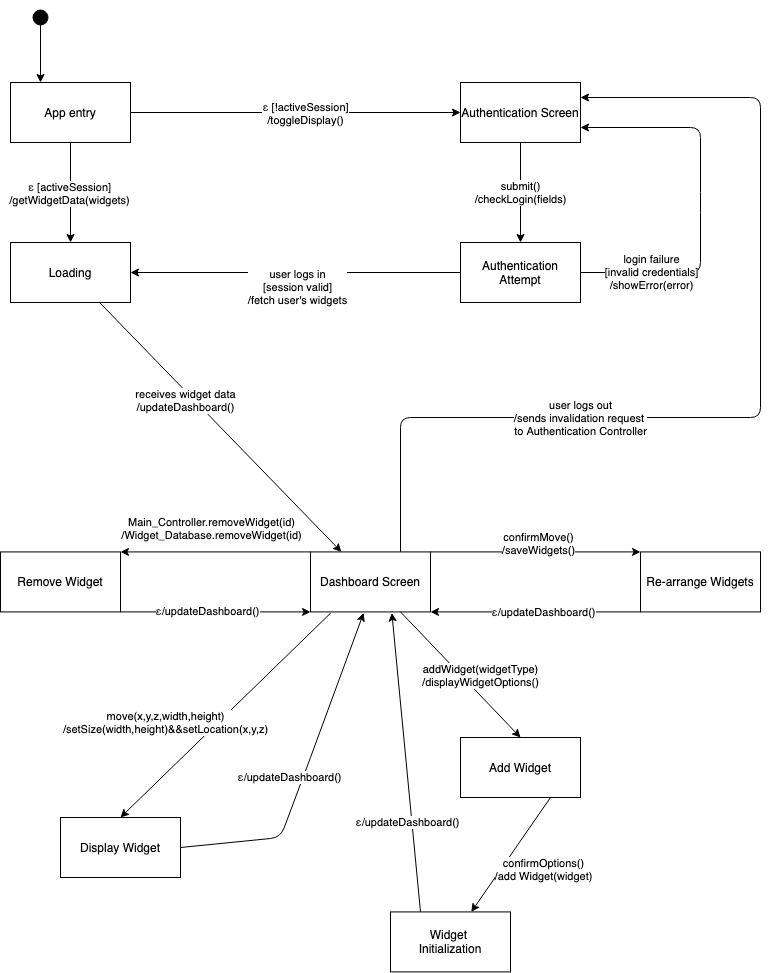
\includegraphics[width=0.95\textwidth]{D3/images/MainController.png}
\end{center}
\caption{Main Controller State Chart}
\label{fig:Main Controller State Chart}
\end{figure}

\subsection{Authentication Controller}
\label{sub:auth_controller_state}
\begin{figure}[H]
\begin{center}
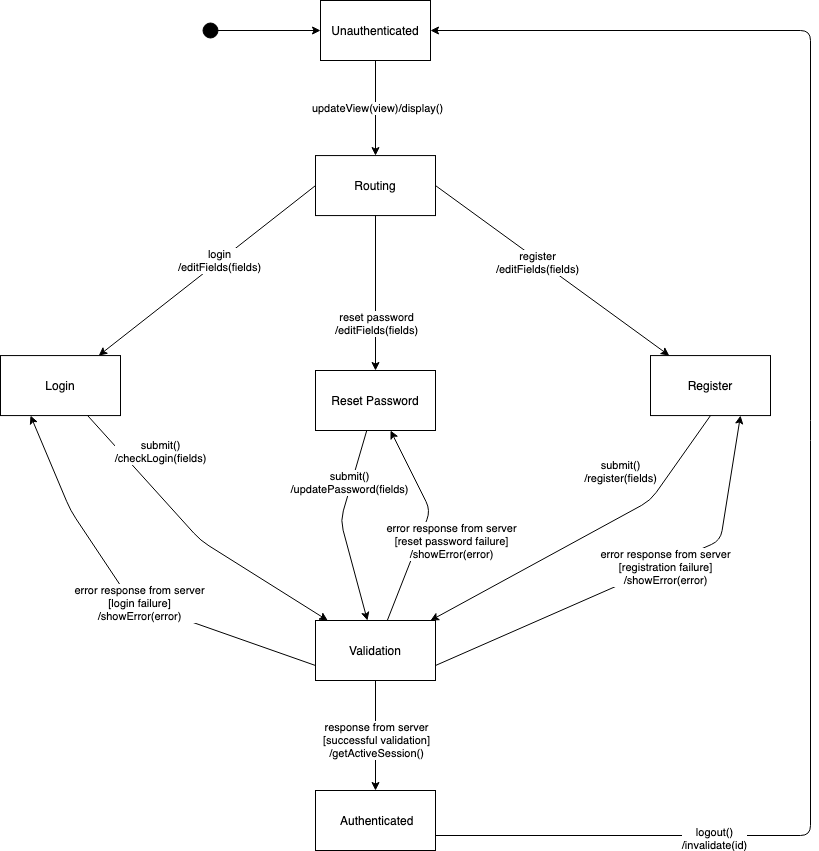
\includegraphics[width=1\textwidth]{D3/images/AuthController.png}
\end{center}
\caption{Authentication Controller State Chart}
\label{fig:Authentication Controller State Chart}
\end{figure}

\subsection{Widget Controller}
\label{sub:widget_controller_state}
\begin{figure}[H]
\begin{center}
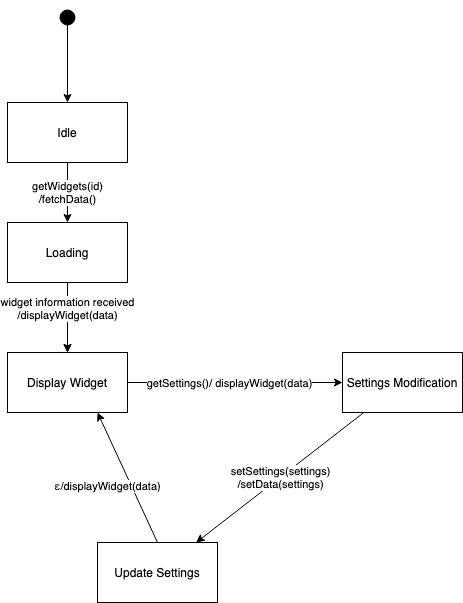
\includegraphics[width=0.95\textwidth]{D3/images/GenericWidgetController.png}
\end{center}
\caption{Generic Widget Controller State Chart}
\label{fig:Widget Controller State Chart}
\end{figure}
% End Section

\section{Sequence Diagrams}
\label{sec:sequence_diagrams}
% Begin Section
\subsection{View Dashboard}
\label{sub:view_dashboard_seq}
\begin{figure}[H]
\begin{center}
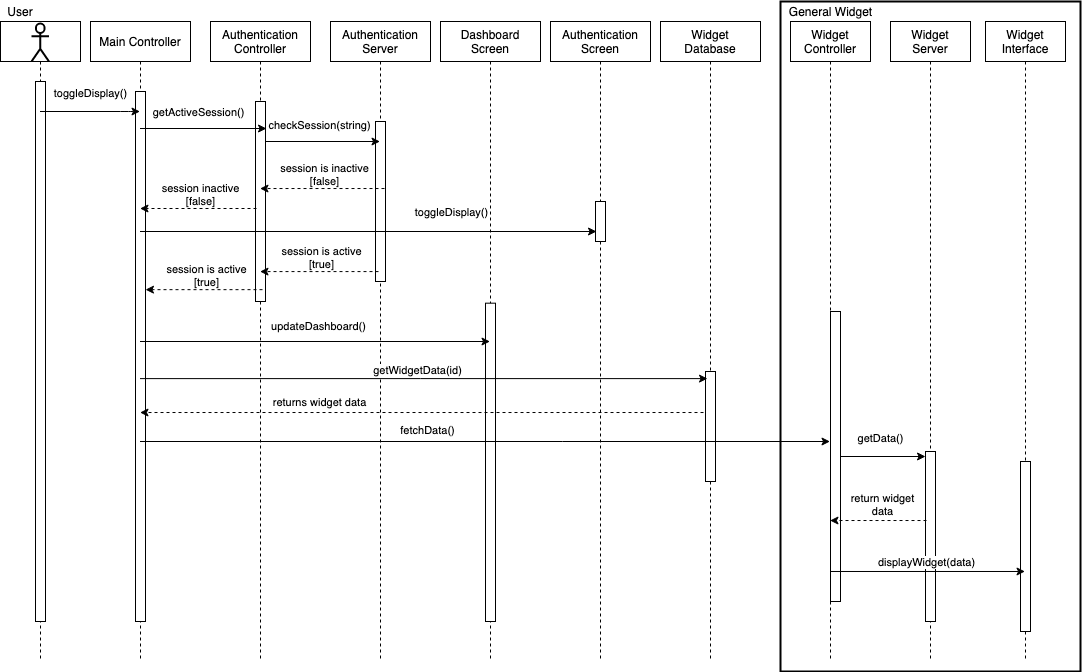
\includegraphics[width=1.25\textwidth, angle=270]{D3/images/ViewDashboardSeq.png}
\end{center}
\caption{Sequence Diagram for Viewing the Dashboard}
\label{fig:View Dashboard}
\end{figure}

\subsection{Remove Widget}
\label{sub:remove_seq}
\begin{figure}[H]
\begin{center}
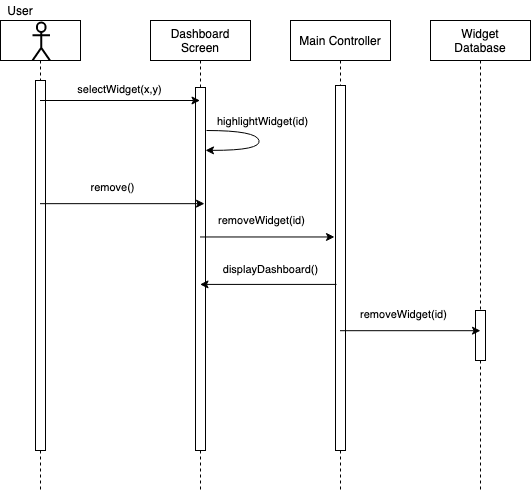
\includegraphics[width=0.95\textwidth]{D3/images/RemoveWidget.png}
\end{center}
\caption{Sequence Diagram for Removing a Widget}
\label{fig:Remove Widget}
\end{figure}

\subsection{Rearrange Widgets}
\label{sub:rearrange_seq}
\begin{figure}[H]
\begin{center}
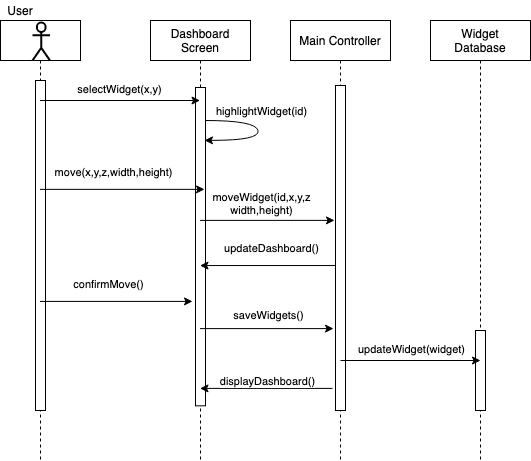
\includegraphics[width=0.95\textwidth]{D3/images/RearrangeWidgets.png}
\end{center}
\caption{Sequence Diagram for Rearranging Widgets}
\label{fig:Rearrange Widget}
\end{figure}

\subsection{Add Widget}
\label{sub:add_widget_seq}
\begin{figure}[H]
\begin{center}
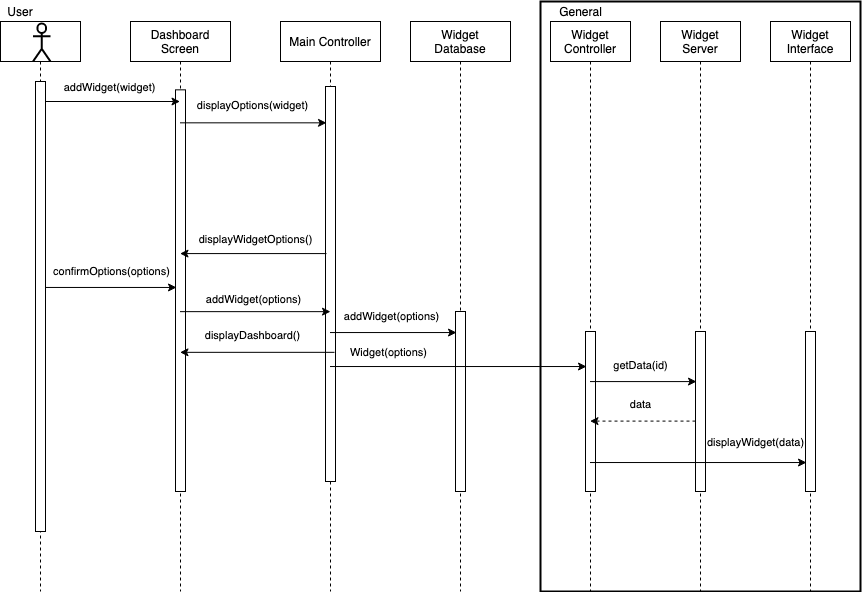
\includegraphics[width=0.95\textwidth]{D3/images/AddWidget.png}
\end{center}
\caption{Sequence Diagram for Adding a Widget}
\label{fig:Add Widget}
\end{figure}

\subsection{Logout}
\label{sub:logout_seq}
\begin{figure}[H]
\begin{center}
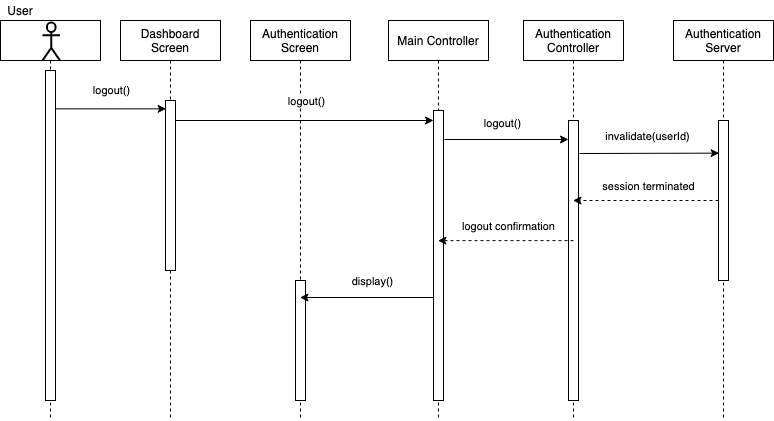
\includegraphics[width=0.95\textwidth]{D3/images/LogoutSeq.png}
\end{center}
\caption{Sequence Diagram for Logging Out}
\label{fig:Logout}
\end{figure}

\subsection{Login}
\label{sub:login_seq}
\begin{figure}[H]
\begin{center}
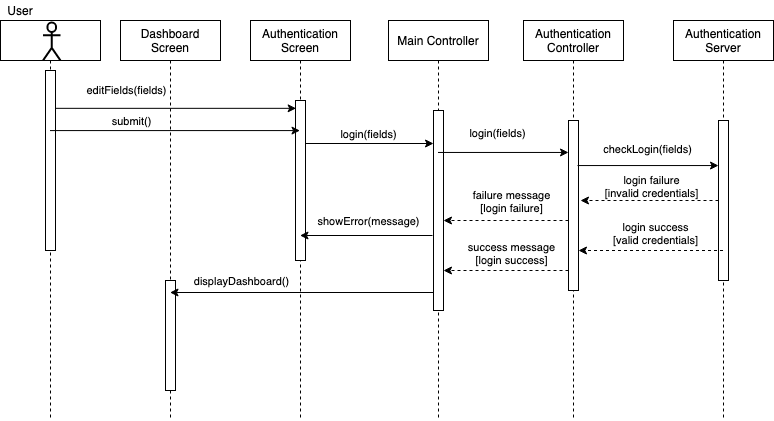
\includegraphics[width=0.95\textwidth]{D3/images/LoginSeq.png}
\end{center}
\caption{Sequence Diagram for Logging In}
\label{fig:Sequence Diagram for login}
\end{figure}

\subsection{Reset Password}
\label{sub:reset_pass_seq}
\begin{figure}[H]
\begin{center}
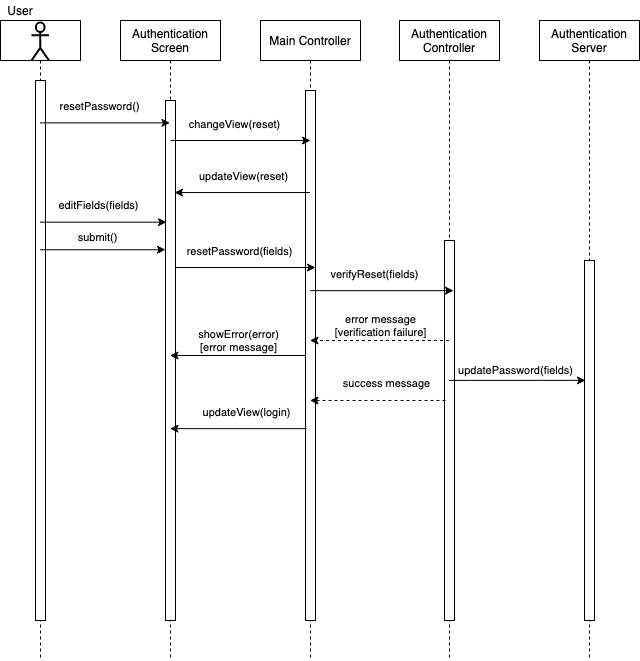
\includegraphics[width=0.95\textwidth]{D3/images/ResetPassword.png}
\end{center}
\caption{Sequence Diagram for Resetting a Password}
\label{fig:Reset Password}
\end{figure}

\subsection{Register}
\label{sub:register_seq}
\begin{figure}[H]
\begin{center}
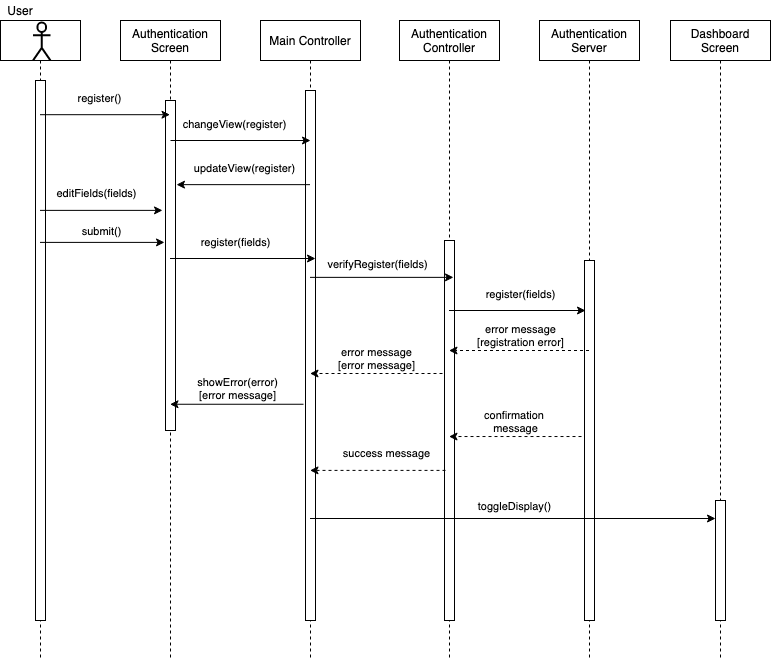
\includegraphics[width=0.95\textwidth]{D3/images/RegisterAccount.png}
\end{center}
\caption{Sequence Diagram for Registering an Account}
\label{fig:Register}
\end{figure}
% End Section

\section{Detailed Class Diagram}
\label{sec:detailed_class_diagram}
% Begin Section
% End Section

\label{sub:detailed class diagram}

\begin{figure}[H]
\begin{center}
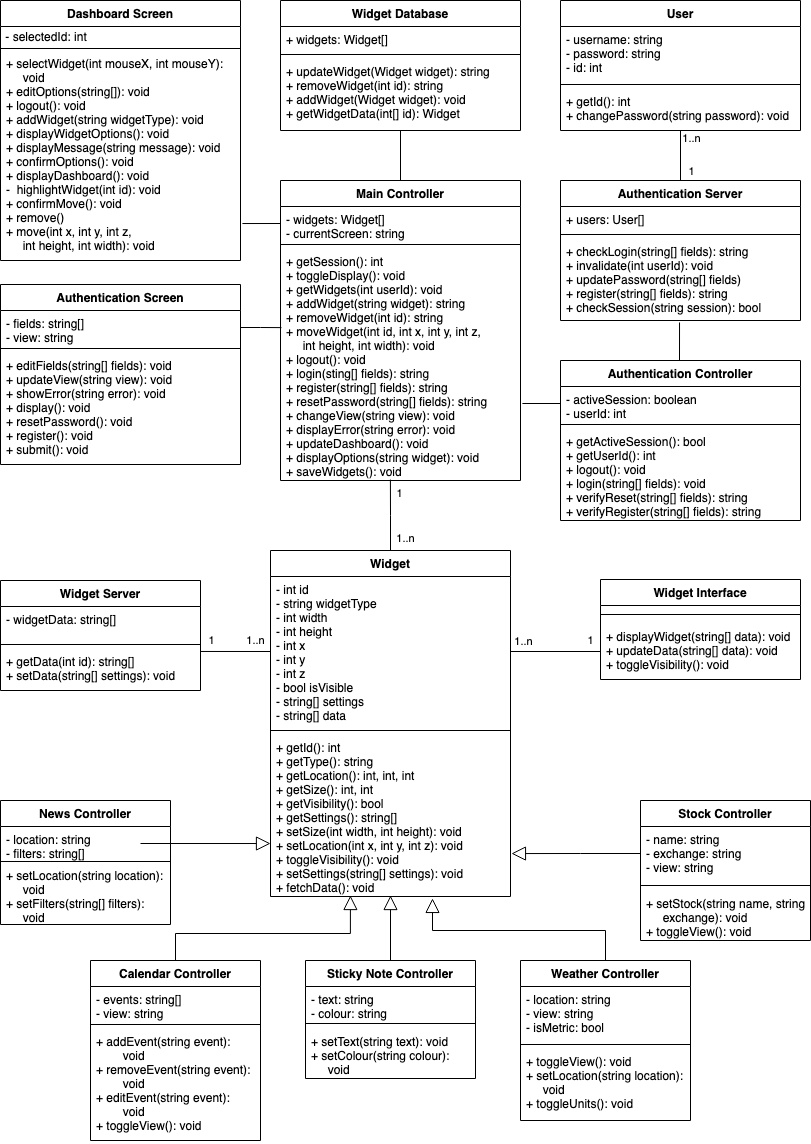
\includegraphics[width=0.9\textwidth]{D3/images/Class Diagram.png}
\end{center}
\caption{Detailed Class Diagram}
\label{fig:Detailed Class Diagram}
\end{figure}

\appendix
\newpage
\section{Division of Labour}
\label{sec:division_of_labour}
% Begin Section
This document was created through a collaborative effort by the whole group, exchanging ideas and filling in sections together. Meetings were held regularly to iterate on this document until an acceptable final version was achieved. By signing this document, the group members certify that this division of labor is fair and accurate.

	\subsection{Signatures}
	\vspace{10ex}
	\begin{center}
	\noindent\begin{tabular}{ll}\\ 
	\makebox[3.5in]{\hrulefill} & \makebox[2in]	\hrulefill \\
	Matthew Paulin & Date\\[15ex]
	\makebox[3.5in]{\hrulefill} & \makebox[2in]	\hrulefill \\		
	Hargun Bedi & Date\\[15ex]
	\makebox[3.5in]{\hrulefill} & \makebox[2in]	\hrulefill \\		
	Dylan Smith & Date\\[15ex]
	\makebox[3.5in]{\hrulefill} & \makebox[2in]	\hrulefill \\		
	Chenwei Song & Date\\[15ex]
	\makebox[3.5in]{\hrulefill} & \makebox[2in]	\hrulefill \\
	Tianzheng Mai & Date\\
	\end{tabular}
	\end{center}
% End Section
\end{document}
%------------------------------------------------------------------------------